\documentclass[10pt,letterpaper]{article}

\usepackage{cogsci}
\usepackage{pslatex}
\usepackage{apacite}

\usepackage{amsmath, amsthm, amssymb}
\usepackage{graphicx}
\usepackage{color}

\newcommand{\TODO}[1]{\textcolor{red}{[TODO: #1]}}

\newcommand{\threshold}[0]{$T=2$}
\newcommand{\betazero}[0]{$\beta_0=683.86,\ 95\%\ \mathrm{CI}\ [601.66, 766.06]$}
\newcommand{\betaone}[0]{$\beta_1=46.01,\ 95\%\ \mathrm{CI}\ [19.71, 72.32]$}
\newcommand{\betatwo}[0]{$\beta_2=63.67,\ 95\%\ \mathrm{CI}\ [57.26, 70.07]$}
\newcommand{\kapb}[0]{$\kappa_b=50.42$}
\newcommand{\kapm}[0]{$\kappa_m=502850.41$}
\newcommand{\kapv}[0]{$\kappa_v=255.60$}
\newcommand{\perr}[0]{$\sigma_p=31.02$}
\newcommand{\sdzero}[0]{$\sigma_0=167.06$}
\newcommand{\sdadj}[0]{$\sigma_{adj}=0.9$}

\newcommand{\HoleResponseCorr}[0]{$r=0.77,\ 95\%\ \mathrm{CI}\ [0.75, 0.78]$}
\newcommand{\HoleRTCorr}[0]{$r=0.67,\ 95\%\ \mathrm{CI}\ [0.64, 0.71]$}
\newcommand{\PaddleCorr}[0]{$r=0.95,\ 95\%\ \mathrm{CI}\ [0.91, 0.97]$}

\newcommand{\AvgResponse}[0]{$53.2\%$}
\newcommand{\AvgCorrect}[0]{$72.4\%$}
\newcommand{\ResponseN}[0]{$N=15216$}
\newcommand{\AvgRT}[0]{$RT=1010.13\ \mathrm{msec},\ 95\%\ \mathrm{CI}\ [997.81, 1022.74]$}
\newcommand{\ResponseFull}[0]{$\chi^2(3)=64.469,p < 0.001$}
\newcommand{\ResponseHoleClass}[0]{$\chi^2(3)=4477.182,p < 0.001$}
\newcommand{\ResponseHoleSize}[0]{$\chi^2(1)=168.598,p < 0.001$}
\newcommand{\RTFull}[0]{$\chi^2(3)=27.146,p < 0.001$}
\newcommand{\RTHoleClass}[0]{$\chi^2(3)=63.611,p < 0.001$}
\newcommand{\RTHoleSize}[0]{$\chi^2(1)=8.981,p < 0.01$}
\newcommand{\RTZeroBounces}[0]{$RT=799.99\ \mathrm{msec},\ 95\%\ \mathrm{CI}\ [783.07, 815.99]$}
\newcommand{\InterceptZeroBounces}[0]{$\beta_0=757.86,\ 95\%\ \mathrm{CI}\ [756.67, 759.05]$}
\newcommand{\RTOneBounces}[0]{$RT=1027.87\ \mathrm{msec},\ 95\%\ \mathrm{CI}\ [1007.75, 1050.46]$}
\newcommand{\InterceptOneBounces}[0]{$\beta_0=894.24,\ 95\%\ \mathrm{CI}\ [891.74, 896.63]$}
\newcommand{\RTTwoBounces}[0]{$RT=1251.20\ \mathrm{msec},\ 95\%\ \mathrm{CI}\ [1225.41, 1276.81]$}
\newcommand{\InterceptTwoBounces}[0]{$\beta_0=1025.80,\ 95\%\ \mathrm{CI}\ [1021.74, 1029.79]$}

\newcommand{\HoleNumFailed}[0]{$N=8$}
\newcommand{\HoleNumIncomplete}[0]{$N=25$}
\newcommand{\HoleNumOk}[0]{$N=320$}
\newcommand{\HoleNumComplete}[0]{$N=328$}
\newcommand{\PaddleNumFailed}[0]{$N=18$}
\newcommand{\PaddleNumIncomplete}[0]{$N=3$}
\newcommand{\PaddleNumOk}[0]{$N=42$}
\newcommand{\PaddleNumComplete}[0]{$N=60$}


% space below "Figure 1: ...", but only for inline figures
%\addtolength{\textfloatsep}{-0.1cm}

\addtolength{\abovecaptionskip}{-0.25cm}
\addtolength{\belowcaptionskip}{-0.5cm}

\title{Think again?\\ Optimal mental simulation tracks problem difficulty}

\author{{\large \bf Jessica B.~Hamrick$^1$ (jhamrick@berkeley.edu),
    Kevin A.~Smith$^2$ (k2smith@ucsd.edu),}\\
    {\large \bf Thomas L.~Griffiths$^1$ (tom\_griffiths@berkeley.edu),
      \& Edward Vul$^2$ (evul@ucsd.edu)}\\
    $^1$University of California, Berkeley, Department of Psychology, Berkeley CA 94720 USA\\
    $^2$University of California, San Diego, Department of Psychology, La Jolla, CA 92093 USA}

\begin{document}

\maketitle

\begin{abstract}
\TODO{In this paper, we investigate the number of simulations that people run when reasoning about a task that requires mental simulation of physics. 
Specifically, we ask the question: do people vary the number of mental simulations that they run depending on the difficulty of the problem?
To answer these questions, we ran a behavioral experiment in which people watched a ball bouncing around in a box, and had to judge whether it would first go through a hole in the wall, or bounce off that wall. 
We varied the difficulty of each trial by changing the size of the holes and the margin by which the ball either went through the hole or missed the hole. 
Following the predictions of the \emph{sequential probability ratio test}, or SPRT \cite{wald1947sequential}, we hypothesized that people should be faster to respond on ``easy'' trials (e.g., where the ball goes directly through the center of a large hole, or hits the wall very far away from the hole), and slower to respond on ``hard'' trials (e.g., where the ball just barely goes through the hole, or just barely misses the hole). 
In brief, we find that judgments of whether the ball goes in and the corresponding response times are well-predicted by a model that combines noisy physical simulation with SPRT.}

\textbf{Keywords:} 
add your choice of indexing terms or keywords; kindly use a
semicolon; between each term
\end{abstract}

\section{Introduction}

%% The question we're interested in: how many simulations do people take?
Imagine you are playing the game Angry Birds, where the goal is to launch a bird to knock down a tower. 
As you aim the bird, you need to predict where the bird will go to decide whether your shot will have the desired effect. 
How do you know where to aim, and how long do you spend thinking about each shot before you take it? 
If you shoot the bird without spending time to consider where it will go, your shot will likely be far off. 
But on the other hand, if you spend too long aiming, over time your predictions will only get marginally better, and you eat into the time you have to play until your next meeting. 
Making this physical prediction requires a tradeoff that underlies many cognitive tasks: spending time and cognitive resources to increase confidence about what will transpire next, versus using that information to make decisions in the moment. 
In this paper, we study whether people efficiently trade off between information seeking and exploitation in a physical prediction task.

Recent research in the domain of physical reasoning has revealed that people make predictions like these by running noisy physical simulations \cite{Smith:2013fc,Battaglia2013,Smith:2013ug,Smith:2013th,Smith:2014tx,Ullman:2014ut,Hamrick:2015}---the ``noisy Newton'' hypothesis \cite{Sanborn2013}. 
However, while this research has investigated the \emph{mechanism} by which people make these types of predictions, there has been very little investigation into \emph{how} people actually use this mechanism. 
In particular, because the simulations are noisy, it may be beneficial to run multiple simulations in order to obtain more accurate predictions.
So, if we are running mental simulations, how to we choose how many simulations to run?

To investigate how many simulations people run, we focus on a dichotomous prediction task---will a ball in motion on a computer screen go through a hole, or miss it?
To model this task, we combine the simulation mechanism of the ``noisy Newton'' hypothesis with a decision strategy for sample-based agents.
Specifically, we consider the \textit{sequential probability ratio test}, or SPRT, in which an agent takes samples that point to one hypothesis or another, and continues to do so until the net samples in favor of one hypothesis reaches a threshold, at which point that hypothesis wins \cite{wald1947sequential}. 
SPRT has been used successfully to explain behavior in a number of decision-making tasks \cite<e.g.>{Gold:2007fo,Ratcliff:2008ux,Bitzer:2014ea}, as it provides an optimal cost-benefit tradeoff between sampling and exploiting information \cite{Wald:1950uw}.

Crucially, the SPRT framework allows us to make testable predictions about how quickly people perform two-alternative forced choice tasks. 
Because it involves sampling until the net evidence reaches a threshold, the number of samples will depend on the variability of the hypotheses. 
If every sample gives the same information (e.g., that the ball goes in the hole), then this net evidence will reach the threshold quickly, and fewer samples will be taken. 
On the other hand, if the samples are more variable, it will take more samples to reach the net evidence threshold. 
Thus, if people are relying on SPRT to decide how many simulations to run, we should observe faster response times for obvious cases (such as the ball hitting the wall far away from the hole) than for ambiguous ones (such as the ball just barely missing the hole).

%% Plan of the paper
In this paper, we first explain the SPRT framework and how it makes predictions about the number of samples required based on variability in sampling. 
Next, we describe an experiment in which we asked participants to respond to the question of, ``will the ball go through the hole?'', and analyze peoples' accuracy and response times. 
We then demonstrate that combining the physical prediction model from \citeA{Smith:2013fc} with SPRT can explain the empirical pattern of accuracy and response times we observed. 
Finally, we discuss the implications of our results on the broader, underlying question: how do people use mental simulation?

\begin{figure*}[t!]
    \begin{center}
        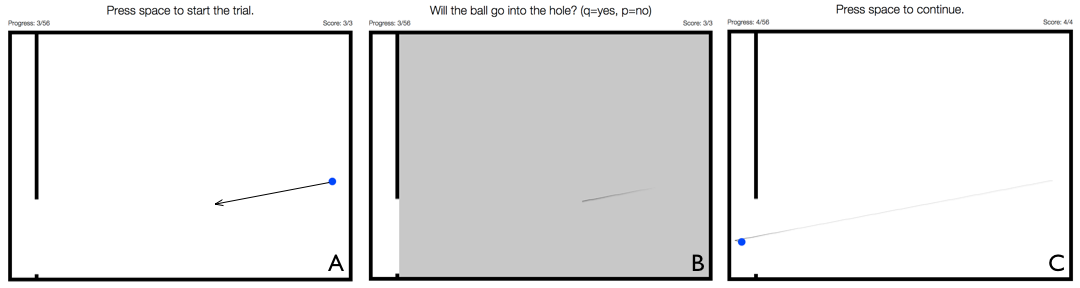
\includegraphics[width=\textwidth]{figures/experiment.png}
        \caption{\textbf{Example experimental trial.} 
        Each panel shows a different part of the trial. 
        \emph{Left:} the initial screen presented to the participant.
        The arrow was not part of the actual stimuli; it has been added to reflect the animation that participants observed after pressing ``space''. 
        \emph{Middle:}  the screen is occluded after observing the stimulus presentation. 
        The faded gray line shows the path the ball took during the initial presentation. 
        \emph{Right:} the final position of the ball, after observing the feedback. 
        As in the middle panel, the faded gray line shows the path of the ball.}
        \label{fig:experiment}
    \end{center}
\end{figure*}

\section{The SPRT strategy}

We consider binary (or two-alternative forced choice) decisions, where an agent must choose one of two hypotheses, $H_0$ or $H_1$. 
The agent may take samples $X_i$ from a Bernoulli distribution parameterized by an unknown parameter $p$ (the probability of sampling evidence for $H_1$), and from these samples estimate the probability that $H_1$ is correct: $\hat{p}=\frac{1}{N}\sum_{i=1}^N X_i$, where $N$ is the total number of samples. 
Then, the decision rule which minimizes the probability of error is $\hat{H}(X_1,\ldots{},X_N)=H_0$ when $\hat{p}<0.5$ and $\hat{H}(X_1,\ldots{},X_N)=H_1$ when $\hat{p}>0.5$.

In the best possible case, the agent takes infinitely many samples and chooses the maximum \emph{a posteriori} (MAP) hypothesis with probability $p$. 
In practice, the agent cannot take infinitely many samples. 
Thus, to determine when to stop sampling (i.e., what the value of $N$ is), the agent continues to sample until the net evidence $Y_N$ reaches some threshold, either $Y_N=T$ to select in favor of $H_1$ or $Y_N=-T$ to select in favor of $H_0$. 
The net evidence is the sum of samples in favor of $H_1$ minus those in favor of $H_0$, or $Y_N=\sum_{i=1}^N 2X_i-1$.

The probability of choosing $H_1$ given that $H_1$ is the MAP hypothesis is:
\begin{equation}
\Pr[\hat{H}(Y_N)=H_1\,|\,H_1]=\frac{p^T}{p^T+(1-p)^T}
\label{eq:pr-choose-h1}
\end{equation}

Given the threshold $T$, the probability of taking $N$ samples and then choosing $H_1$ is:
\begin{multline}
\Pr[N,H_1\,|\,T,p]=\left(\frac{2^N}{2T}\right)p^{\frac{N+T}{2}}(1-p)^{\frac{N-T}{2}}\cdot{}\\
\sum_{\nu=1}^{2T-1}\cos\left(\frac{\nu\pi}{2T}\right)^{N-1}\sin\left(\frac{\nu\pi}{2T}\right)\sin\left(\frac{\nu\pi}{2}\right)
\end{multline}
for $N\geq T$ and where $N$ is of the same parity as $T$ \cite[ch.~XIV, eq. 5.7]{Feller:1968ut}. 
Because we are dealing with binary hypotheses, the marginal probability of $N$ samples is then $\Pr[N\,|\,T,p]=\Pr[N,H_1\,|\,T,p]+\Pr[N,H_1\,|\,T,1-p]$.
So, the expected number of samples for a particular decision is:
\begin{equation}
\mathbb{E}[N\,|\,T,p]=\sum_{N=T}^\infty N\cdot{}\Pr[N\,|\,T,p]
\label{eq:expsamp}
\end{equation}

To summarize thus far, Equations \ref{eq:pr-choose-h1} and \ref{eq:expsamp} give us a formal hypothesis for what decisions people make, and how long they choose to make them. 
In the next section, we present an experiment to empirically test this hypothesis.

\section{Experiment}

In order to determine whether people take physical simulation samples in a way consistent with SPRT, we designed an experiment in which people made a binary judgment about what will happen in the future.
Specifically, we asked participants to reason about whether a ball traveling across a computer screen would go through a hole or not (see Figure \ref{fig:experiment}).
We designed the trials such that some were harder than others by varying the margin by which the ball either missed or went through the hole.
According to SPRT, people should be faster to respond on ``easy'' trials (e.g., where the ball goes directly through the center of a large hole, or hits the wall very far away from the hole), and slower to respond on ``hard'' trials (e.g., where the ball just barely goes through the hole, or just barely misses the hole).

\subsection{Participants}

We recruited \HoleNumComplete{} participants on Amazon's Mechanical Turk using the psiTurk \cite{McDonnell12} experimental framework.
Participants were treated in accordance with UC Berkeley IRB standards and were paid \$0.60 for approximately 6.5 minutes of work.
Participants were randomly assigned to one of eight conditions, which determined which stimuli they judged based on a latin-square design (see Stimuli). 
Additionally, we excluded \HoleNumFailed{} participants from analysis for answering incorrectly on more than one control trial (see Stimuli), leaving a total of \HoleNumOk{} participants.

\subsection{Procedure}

On each trial, participants were shown the scene, including the initial position of the ball and the location of the hole. 
Participants were instructed to press the ``space'' key to begin the trial. 
Immediately upon pressing ``space'', the initial stimulus presentation began. 
As soon as the initial stimulus animation concluded, a gray box was drawn over the screen, occluding the ball (but not the line depicting the path it had traveled so far; this was left in as a reminder to participants of where the ball had come from). 
Participants were asked, ``will the ball go in the hole?'', and were instructed to press `q' to respond in the affirmative, and `p' to respond in the negative. 
Immediately after responding, text appeared saying ``Correct!'' or ``Incorrect.'', depending on the participants' response.
Additionally, the gray occluder was removed, and participants were shown feedback animation of the path of the ball.
After the feedback animation was complete, the final frame of the animation remained on the screen until participants pressed ``space'' to advance to the next trial.

During the experiment, participants made judgements on 48 experimental trials, presented in a random order, as well as eight control trials, which were also shown in a random order, but interspersed with the experimental trials such that every 8th trial was a control trial.
In addition, participants were given seven instruction trials prior to the experiment to familiarize them with the procedure.

\subsection{Stimuli}

The stimuli consisted of animations depicting a blue ball with a radius of 10px bouncing around in a box with dimensions 900px $\times$ 650px.
All stimuli consisted of two separate animations.
The first was the stimulus presentation, which had a duration of 0.775 seconds and depicted the ball moving in a particular direction.
The second animation was the feedback, which picked up immediately where the first animation left off, and which had a duration of 1.5 seconds and depicted the ball either going into the hole or bouncing off the wall that contained the hole.%
\footnote{To enforce the constraint that the ball always travel the same distance during the feedback animation, the $x$-coordinate of the wall with the hole in it was allowed to vary across stimuli.}
During the feedback animation, the ball could bounce on the other walls either 0, 1, or 2 times before going into the hole or hitting the wall with the hole in it.
In both animations, the ball had a velocity of 400px/s.
Additionally, in the animations, the path that the ball had traveled so far was drawn with a faded gray line (see Figure \ref{fig:experiment}).

There were 48 different initial animations, equally balanced by number of bounces during feedback (16 each for 0, 1, and 2 bounces). 
For each of these initial animations, there were four different trial types and two different hole sizes, giving a total of eight versions of each stimulus. 
The four trial types were: ``far in'' (FI), where the ball went directly through the center of the hole; ``far miss'' (FM), where the ball missed the hole by a wide margin; ``close in'' (CI), where the ball just barely went through the hole; and `` close miss'' (CM), where the ball just barely missed the hole. 
The two hole sizes were 100px and 200px.

In order to ensure that participants never saw the same initial animation twice, we used a latin-square design of Initial Animation $\times$ Trial Type $\times$ Hole Size.
Thus, each participant saw each initial animation exactly once, each trial type exactly 12 times, and each hole size exactly 24 times.
This also ensured that the ball would go through the hole exactly half the time, so that participants would not be biased to respond either way based on statistical contingencies.

In addition to the 48 experimental trials, there were seven instruction trials and eight control trials, which were the same for all participants.
The control trials were designed to be extremely easy and were either of type ``straight hit'' (with a hole size of either 300px or 350px) or ``far miss'' (with a hole size of 100px).
Thus, participants saw a total of 63 trials throughout the experiment.

\begin{figure*}[t]
    \begin{center}
        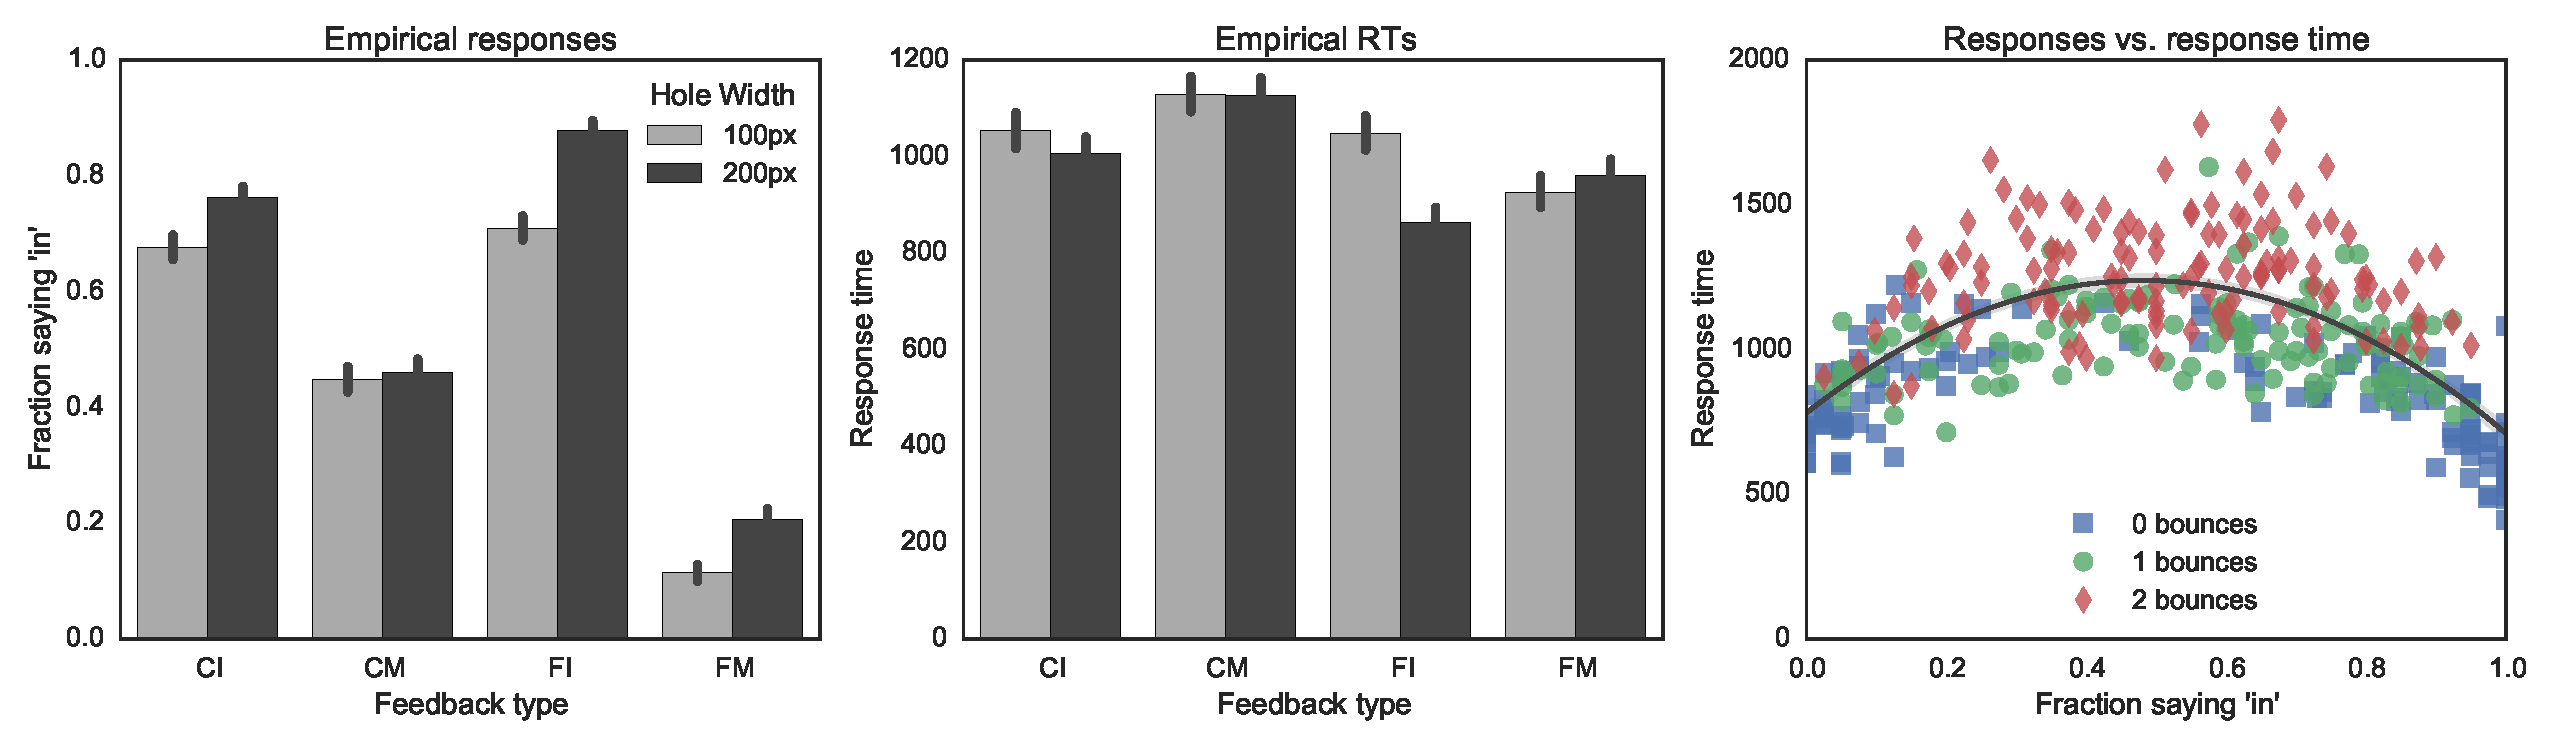
\includegraphics[width=\textwidth]{figures/hole_empirical_results.pdf}
        \caption{\textbf{Response times as a function of response.} \emph{Left:} each bar shows the proportion of participants saying that the ball will go in the hole for a particular trial type ($x$-axis) and hole size (color). \emph{Middle:} like the left subplot, but the $y$-axis shows bootstrapped logarithmic means of response times. \emph{Right:} each point corresponds to a different stimulus, trial type, and hole size.  The $x$-axis is the proportion of participants saying the ball will go in the hole, and the $y$-axis is the logarithmic mean response time. The black line indicates a 2nd-order polynomial fit between responses and response times and the shaded gray region indicates the 95\% confidence interval around the fit.}
        \label{fig:pct-vs-rt}
    \end{center}
\end{figure*}

\subsection{Results}

\subsubsection{Responses}

On average, participants were correct \AvgCorrect{} of the time and responded that the ball would go in the hole \AvgResponse{} of the time (\ResponseN{}), excluding catch trials.
There was a significant effect of trial type on participants' responses (\ResponseHoleClass{}) as well as a significant effect of hole size (\ResponseHoleSize{}).
Additionally, there was an interaction between trial type and hole size (\ResponseFull{}).
For three out of the four trial types, there was a significant difference between responses for the two different hole sizes (for CI, \ResponseCIttest{}; for FI, \ResponseCIttest{}; and for FM, \ResponseFMttest{}), with the exception being the ``close miss'' (CM) trials (\ResponseCMttest{}).
Figure \ref{fig:pct-vs-rt}A shows responses as a function of trial type and hole size.

\subsubsection{Response times}

For all analyses of response time, we computed averages using bootstrapped logarithmic means (exponential of the mean of the log response times), using 1000 bootstrap samples.
Participants had an average response time of \AvgRT{}, excluding catch trials.
There were significant effects of both trial type (\RTHoleClass{}) and hole size (\RTHoleSize{}) on response time, as well as an interaction between trial type and hole size (\RTFull{}).
However, there was only evidence for a difference in reaction times by hole size in the case of the ``far in'' (FI) trials (\ResponsetimeFIttest{}), in which the ball went straight through the center of the hole (for CI, \ResponsetimeCIttest{}; for CM, \ResponsetimeCMttest{}; and for FM, \ResponsetimeFMttest{}).
Figure \ref{fig:pct-vs-rt}B shows the response times as a function of trial type and hole size.

\subsubsection{Relationship of responses to reaction time}

As shown in Figure \ref{fig:pct-vs-rt}C, we found a clear effect of certainty on people's response times.
In particular, on trials when there was more agreement amongst participants (the fraction saying `in' is closer to $0$ or $1$), participants were faster to respond than when responses were more variable.
This tradeoff mirrors the same tradeoff found in SPRT: decisions for which $p\approx0.5$ are slower, because it on average takes more samples to get to one threshold versus the other.
Thus, it is clear that people are not spending a fixed amount of time thinking about each trial; rather, they spend more time thinking about the ``hard'' trials than the ``easy'' trials.

In addition, we found that response time is affected by the number of bounces during feedback.
Participants were fastest to respond on trials with zero bounces (\RTZeroBounces{}), slower to respond on trials with once bounce (\RTOneBounces{}), and slowest to respond on trials with two bounces (\RTTwoBounces{}).
While this may be partially modulated by difficulty---people make more variable predictions as bounces are added \cite{Smith:2013fc}, and more variable trials have longer reaction times---there appears to be an additional time cost.
For each number of bounces, we fit participants' response times to a second-order polynomial function of their responses.
From these fits, we see that the intercepts are significantly different across the different numbers of bounces: for zero bounces, the intercept was \InterceptZeroBounces{}; for one bounce, \InterceptOneBounces{}; and for two bounces, \InterceptTwoBounces{}.
This suggests that it takes additional time to resolve a collision between the ball and a wall in the course of a simulation.

\section{Modeling mental sampling}

In the previous section, we presented an experiment in which participants had to judge whether a ball would go through a hole.
The results indicate a clear relationship between people's responses and response times---one which appears qualitatively similar to the one we would expect from SPRT.
In this section, we flesh out our hypothesis that people predict where the ball will go by running noisy physical simulations, and that they run a variable number of simulations on each trial based on SPRT principles \cite{wald1947sequential}.

\subsection{The physical simulator}

There is a growing body of evidence that people reason about physical scenes by running noisy simulations.
This hypothesis, referred to as the ``noisy Newton'' hypothesis, states that people have approximate knowledge of physical laws instantiated in a runnable model of intuitive physics.
Using this model, they can extrapolate the future of physical scenes by running a series of noisy simulations \cite{Smith:2013fc,Battaglia2013,Smith:2013ug,Smith:2013th,Smith:2014tx,Ullman:2014ut,Hamrick:2015}.
In particular, \citeA{Smith:2013fc} investigated the various sources of uncertainty in these simulations, finding that people's judgments were best captured by a model that took into account both perceptual uncertainty (noise in exactly where objects are and their motion trajectories) and dynamic uncertainty (stochastic noise added to account for unknowable variation in motion---e.g., a textured floor would cause a ball rolling along it to deviate from a straight line).

Specifically, \citeA{Smith:2013fc} asked people to catch a ball like the one in Figure \ref{fig:experiment} using a paddle that could move up and down along the $y$-axis.
In order to predict where people would place the paddle on each trial, their model incorporated uncertainty in its physical simulations through five parameters: perceptual uncertainty over the position of the ball ($\sigma_p$), uncertainty in the initial direction of velocity ($\kappa_v$), ongoing uncertainty in the direction of movement ($\kappa_m$), uncertainty in the bounce angle ($\kappa_b$), and a ``center bias'' reflecting a bias for people to respond more towards the center of the $y$-axis ($\sigma_0$).

Here, we used the model of \citeA{Smith:2013fc} to describe how people simulate individual possible physical events.
Because the hole-choice experiment was performed online, we performed an online replication of that experiment to set model parameters (see the Appendix for details).
Thus, the physical prediction parameters were set independently of the results of the experiment in this paper.

\subsection{The SPRT sampler}

\begin{figure}[t]
    \begin{center}
        \includegraphics[width=0.45\textwidth]{figures/model_rt_results.pdf}
        \caption{\textbf{Model vs. human response times.} Each point corresponds to a different stimulus, trial type, and hole size; color and shape indicate the number of times the ball bounced during feedback. The $x$-axis is the fitted model response times, and the $y$-axis is the logarithmic mean response times of participants.}
        \label{fig:model-rt-results}
    \end{center}
\end{figure}

The physical prediction model provides a posterior predictive distribution of where the ball will be when it encounters the plane of the wall.
However, it is possible that the participants in the auxiliary experiment used more than one sample to determine where the ball would go.
Assuming they took on average $M$ samples, then the standard deviation we estimate using the physical simulator ($\sigma_{judgments}$) is not equal to the standard deviation of distributions of simulations ($\sigma_{sims}$), but is instead related by the equation: $\sigma_{sims} = \sigma_{judgments} / \sqrt{M}$.
Therefore, we allowed for one free parameter to adjust this variance such that $\sigma_{adj}=\sqrt{M}$.

If sampling pulls from this distribution, the probability of a ball going `in' ($H_1$) on any given sample is simply the density of the probability distribution that overlaps with the hole ($p$).
So, for a given threshold $T$, we can calculate the expected number of samples for any trial using equation \ref{eq:expsamp}.

\subsection{Modeling reaction time}

If we assume that every sample takes the same amount of time, response times as predicted by the model should be directly proportional to $\mathbb{E}[N\,|\,T,p]$.
However, we found the number of bounces to be an extremely strong predictor of response time: each additional bounce adds a constant amount of time to the response.
To account for this, our final response time equation incorporated the number of bounces, $B$, as follows:
\begin{equation}
RT = \beta_0 + (\beta_1 + \beta_2\cdot{}\mathbb{E}[B]) \cdot{}\mathbb{E}[N\,|\,T,p]
\label{eq:rt}
\end{equation}

To compute this equation, we used the physical simulation model to determine $\mathbb{E}[B]$ as the average number of times the ball bounced across all model simulations.
We then fit all parameters ($T$, $\sigma_{adj}$, $\beta_0$, $\beta_1$, and $\beta_2$) to minimize sum squared error between modeled and observed reaction times, using $n=10000$ samples from the physical simulation model.
The best fitting values were: \threshold{}, \sdadj{},\footnote{If \sdadj{}, then $M<1$. How could people be taking fewer than one sample?
We suspect that $\sigma_{adj}<1$ because the model actually overestimates the standard deviation; thus, $\sigma_{adj}$ is adjusting for both the inflated uncertainty in the model as well increased certainty in people's judgments on the paddle task.} \betazero{}, \betaone{}, and \betatwo{}.

\subsection{Results}

The fitted model explains participants' judgments of whether the ball would go in the whole very well (\HoleResponseCorr{}, see Figure \ref{fig:model-response-results}), and can additionally account for how quickly participants responded to trials (\HoleRTCorr{}, see Figure \ref{fig:model-rt-results}).
Even if the number of bounces is not included, the SPRT model with \threshold{} is able to account for a moderate amount of the variance in response times (\NoBouncesHoleRTCorr{}).
In contrast, a simpler model that takes only a single sample each time (equivalent to SPRT with $T=1$) does slightly better at explaining people's responses (\RawHoleResponseCorr{}) but cannot explain the variation in response times beyond the number of bounces.

\section{Discussion}

In this paper, we asked the question: how many simulations do people run?
We hypothesized that although people probably take a very small number of samples \cite{Vul:2014ba}, people still vary the number of samples that they take in order to exploit the fact that some judgments are easier to make than others.
Specifically, we hypothesized that people take samples in a manner consistent with the SPRT strategy, in which evidence for hypotheses is accumulated until one hypothesis has a fixed amount of evidence over the other.

In addition, the parameters of the sampling process can further inform us about how people accomplish physical prediction.
The best fitting threshold was \threshold{}, suggesting people gather little information before making a decision (in line with the theory of \cite{Vul:2014ba}, see the Discussion).

\begin{figure}[t]
    \begin{center}
        \includegraphics[width=0.45\textwidth]{figures/model_response_results.pdf}
        \caption{\textbf{Model vs. human judgments.} Each point corresponds to a different stimulus, trial type, and hole size. The $x$-axis is the probability the model says the ball will go in the hole, and the $y$-axis is the proportion of participants saying the ball will go in the hole.}
        \label{fig:model-response-results}
    \end{center}
\end{figure}

\TODO{MOVE THIS TO THE DISCUSSION TO EXPLAIN THE LOW THRESHOLD WE FIND: According to previous research by \citeA{Vul:2014ba}, a sample-based agent should only take a small number of samples before making a judgment so long as there is any cost to taking samples---perhaps even just one. While taking a single sample clearly provides a worse chance of making a good decision than taking multiple samples, over the long run, taking a small number of samples maximizes expected utility across a large number of judgments. Does this story also hold true for mental simulations? There is some evidence that points to ``yes'': \citeA{Battaglia2013} analyzed the variability of people's responses in tasks concerning towers of building blocks, and found that participants seemed to use between three and seven samples per judgment.}

The results of Experiment 1 paint a clear picture that people \emph{do} vary the number of samples they take, as evidenced by the increase in response time on ``hard'' trials (i.e., trials which people are less confident about).
This pattern of taking longer to respond on trials with $p\approx 0.5$ is qualitatively consistent with the strategy of SPRT.
To demonstrate quantitatively that SPRT is a good account for people's responses, we formulated a model of people's responses based on the ``Noisy Newton'' hypothesis and SPRT.
In Experiment 2, replicated the experiment from \citeA{Smith:2013fc}, and used the results to fit our model.
Comparing people's responses and response times in Experiment 1 to those of the model, we found an extremely strong fit, suggesting that people are relying both on simulations from approximate physical simulations, and that they vary the number of simulations that they run according to SPRT.

\section{Appendix}

In order to fit the parameters for the physical simulation model, we ran an online replication of the experiment from \citeA{Smith:2013fc}.

\subsection{Participants}

We recruited \PaddleNumComplete{} participants on Amazon's Mechanical Turk using the psiTurk \cite{McDonnell12} experimental framework.
Participants were treated in accordance with UC Berkeley IRB standards and were paid \$0.60 for approximately 5 minutes of work.
Additionally, we excluded \PaddleNumFailed{} participants from analysis for failing to catch the ball on more than one control trial, leaving a total of \PaddleNumOk{} participants.

\subsection{Stimuli}

The stimuli were modified versions of those used Experiment 1, with two major differences.
First, instead of a wall with a hole in it, there was a paddle of length 100px that could move up and down the $y$-axis.
Second, there was no feedback animation; instead, there was just a single feedback image corresponding to the last frame of the feedback animation.
Because there was no feedback animation, there were only 48 stimuli (corresponding to the stimulus presentation animations from Experiment 1), plus the seven instruction trials and eight catch trials.

\subsection{Procedure}

Like Experiment 1, the experiment was divided into two phases: the training phase (consisting of seven trials), and the experimental phase (consisting of the 48 experimental trials, with the eight control trials evenly interspersed).
On each trial, participants were shown the scene, including the initial position of the ball and the location of the hole.
The paddle begin at the center of the $y$-axis, and was freely moveable along the $y$-axis from the very beginning of the trial.
Participants were instructed to press ``space'' to begin the trial. 

As in Experiment 1, immediately upon pressing ``space'', the initial stimulus presentation began, after which an occluder appeared.
However, unlike Experiment 1, as soon as the occluder appeared, a timer also appeared and begin counting down for 2 seconds.
During this time, participants had to move the paddle to try to catch the ball in the position it would be when the timer was up.
When the timer countdown finished, the paddle froze at its current location, and the occluder was removed and the full path of the ball revealed.
If the ball was on the paddle, then participants were told, ``You caught the ball!''.
If the ball was not on the paddle, participants were told ``Oops, you didn't catch the ball.''
Participants were then instructed to press ``space'' to continue, at which point the next trial would begin.

\subsection{Results}

We fit the model parameters of $\sigma_p$, $\kappa_v$, $\kappa_m$, $\kappa_b$, and $\sigma_0$ to particant's responses \cite<for details, see>{Smith:2013fc}, finding the best fitting parameters to be \perr{}, \kapv{}, \kapm{}, \kapb{}, and \sdzero{}. 
With these parameters, we found very similar results to those from \citeA{Smith:2013fc}.
In particular, we found a correlation of \PaddleCorr{} between the model's predicted means of where the ball would end up and people's average location of the paddle.

\bibliographystyle{apacite}

\setlength{\bibleftmargin}{.125in}
\setlength{\bibindent}{-\bibleftmargin}

\bibliography{references}

\end{document}
